%%%%%%%%%%%%%%%%%%%%%%%%%%%%%%%%%%%%%%%%%
% a0poster Portrait Poster
% LaTeX Template
% Version 1.0 (22/06/13)
%
% The a0poster class was created by:
% Gerlinde Kettl and Matthias Weiser (tex@kettl.de)
% 
% This template has been downloaded from:
% http://www.LaTeXTemplates.com
%
% License:
% CC BY-NC-SA 3.0 (http://creativecommons.org/licenses/by-nc-sa/3.0/)
%
%%%%%%%%%%%%%%%%%%%%%%%%%%%%%%%%%%%%%%%%%

%----------------------------------------------------------------------------------------
%	PACKAGES AND OTHER DOCUMENT CONFIGURATIONS
%----------------------------------------------------------------------------------------

\documentclass[a0,portrait]{a0poster}
\usepackage{multicol}
\usepackage[svgnames]{xcolor}
\usepackage{times}
\usepackage{graphicx}
\graphicspath{{figures/}}
\usepackage{booktabs}
\usepackage[font=small,labelfont=bf]{caption}
\usepackage{amsfonts, amsmath, amsthm, amssymb}
\usepackage{wrapfig}
\usepackage{indentfirst}
\usepackage{enumitem}
\usepackage{tikz}
\usetikzlibrary{shapes.geometric, arrows, positioning, fit, backgrounds}


\usepackage{fontspec}
\usepackage[english, bulgarian]{babel}
\usepackage{polyglossia}

\newfontfamily{\cyrillicfont}{NewCM10-Regular} 
\setdefaultlanguage{english}
\setotherlanguages{russian}
%https://tex.stackexchange.com/a/669979

\usepackage[style=authoryear,backend=biber,heading=bibintoc]{biblatex}
\addbibresource{references.bib}
\usepackage{caption}
\newenvironment{Figure}
  {\par\medskip\noindent\minipage{\linewidth}}
  {\endminipage\par\medskip}
%https://tex.stackexchange.com/a/12289

% Define ARDC colors
\definecolor{ARDCBlue}{RGB}{0,159,218}
\definecolor{ARDCPink}{RGB}{236,0,140}
\definecolor{ARDCYellow}{RGB}{255,194,14}
\definecolor{ARDCPurple}{RGB}{146,39,143}
\definecolor{DarkGrey}{RGB}{64,64,64}

% Set margins
\setlength{\topmargin}{2cm}
\setlength{\oddsidemargin}{2cm}
\setlength{\evensidemargin}{2cm}
\setlength{\textwidth}{0.95\paperwidth}
\setlength{\textheight}{0.95\paperheight}
\setlist[enumerate]{leftmargin=2em}

% Increase first-line indent
\setlength{\parindent}{2em}


% \setmainfont{Gentium}

% \usepackage{fontspec}
\setmainfont{TeX Gyre Termes}
% https://tex.stackexchange.com/questions/639067/defining-a-fallback-font-for-all-missing-characters


\begin{document}

%----------------------------------------------------------------------------------------
% POSTER HEADER
%----------------------------------------------------------------------------------------
\noindent\begin{minipage}[t]{\linewidth}
\Huge \color{ARDCBlue} \textbf{The Research Activity Identifier (RAiD):} \color{Black}\\[0.3cm]
\LARGE\textit{System architecture, metadata schema, workflows, and examples}\\[1cm]
\end{minipage}

\noindent\begin{minipage}[t]{0.75\linewidth}
\Large \textbf{Shawn Ross\textsuperscript{1}, Natasha Simons\textsuperscript{1}, Rob Leney\textsuperscript{1}, Steffen Weidenhaus\textsuperscript{1}}\\[0.5cm]
\large \textsuperscript{1}Australian Research Data Commons, Australia
\end{minipage}%
\begin{minipage}[t]{0.25\linewidth}
\raggedleft
\raisebox{\dimexpr-\height+\ht\strutbox\relax}{
\includegraphics[width=0.95\linewidth]{ARDC logo - RGB.png}}
\end{minipage}

\vspace{1cm}

\setlength{\columnsep}{2cm}
\begin{multicols}{2}

%----------------------------------------------------------------------------------------
% BACKGROUND
%----------------------------------------------------------------------------------------
\color{ARDCPink}
\section*{\LARGE Background}
\color{DarkGrey}
\large{
RAiD is a persistent identifier for research projects, which links a project’s organisations, people, inputs and outputs, as well as providing other key information about a research project. It is governed by ISO 23527:2022 with the ARDC as the global Registration Authority and various regional Registration Agencies (currently the ARDC in Australia and New Zealand and SURF Netherlands in Europe). It features prominently in the Australian National PID Strategy. RAiDs reduce the administrative burden of research project management, facilitate reporting of research outputs and impacts, and make research more transparent by exposing a project’s make-up and how it changes over time. Over the past two years, RAiD has been rebuilt and is now in production, both in Australia and overseas. 

This poster presents a technical overview of RAiD, including system architecture, key RAiD features, an overview of the metadata schema, a workflow diagram for obtaining a RAiD, and an example RAiD.
}

%----------------------------------------------------------------------------------------
% Key RAiD features
%----------------------------------------------------------------------------------------

\color{ARDCYellow}
\section*{\LARGE Key RAiD features}
\color{DarkGrey}
\large{
RAiD has been designed from the ground up as a dedicated research project identifier. In addition to serving as a PID for projects, it is also a registry and a collaborative metadata management system.
}

\vspace{2cm}



%----------------------------------------------------------------------------------------
% Technical technical implementation
%----------------------------------------------------------------------------------------
\color{ARDCYellow}
\section*{\LARGE RAiD technical implementation}
\color{DarkGrey}
\large{
Each RAiD Registration Agency runs an instance of the RAiD Service, federated into the global RAiD System. It is designed to be scalable and re-deployable. 
}

% ---------------------------
% RAiD Basic Architecture
% ---------------------------
% Add vertical space before the diagram
\vspace{2cm}


\begin{Figure}
  \centering
  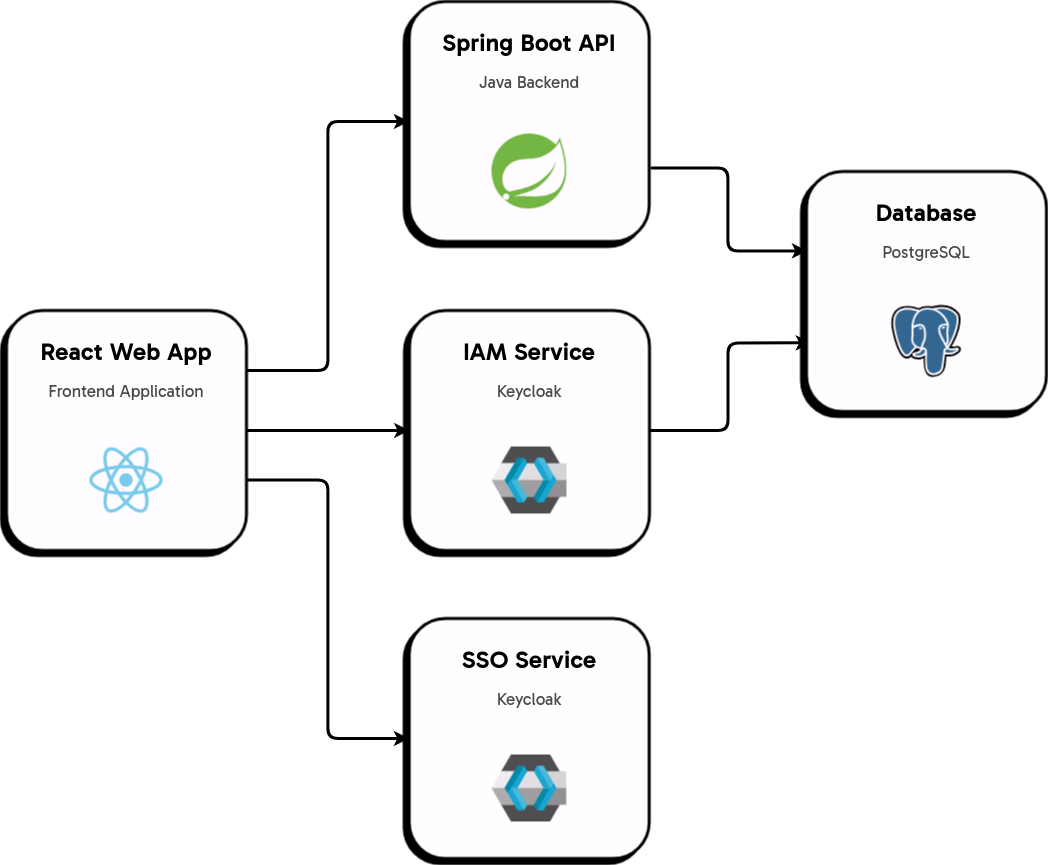
\includegraphics[width=\linewidth]{figures/20241023-raid-architecture-appflow-basic.png}
  \captionof{figure}{RAiD is built using React, Spring Boot, Keycloak, and PostgreSQL.}
  \label{basic-architecture}
\end{Figure}


% ---------------------------
% End RAiD Basic Architecture
% ---------------------------


%----------------------------------------------------------------------------------------
% RAID Metadata schema
%----------------------------------------------------------------------------------------
\color{ARDCPurple}
\section*{\LARGE RAiD metadata schema}
\color{DarkGrey}
\large{
The RAiD Metadata Schema underpins how RAiDs are identified, minted, resolved, and updated. divided into 'Core', 'Extended', and 'Local' components. 

\textbf{Core components} refer to metadata properties and associated controlled lists that are standardised across all RAiD Registration Agencies. If a Registration Agency uses its own controlled lists, it must provide a crosswalk to the RAiD’s standardised core terms.

\textbf{Extended components} are properties that are standardised across all Registration Agencies, but associated controlled lists may vary. A Registration Agency may use its own controlled lists if it publishes each list in a machine-readable format (preferably on a vocabulary service) and registers the controlled list(s) with the ARDC. 

\textbf{Local components} are properties and controlled lists that are entirely under the control of a Registration Agency, and only need to be reported to the ARDC annually or whenever major changes are made. Local properties can be tailored to meet the needs of the research community served by the Registration Agency. 

A mechanism exists to enable useful local metadata to be promoted into extended metadata, or extended into core metadata.
}

\vfill

%----------------------------------------------------------------------------------------
% RAID Example
%----------------------------------------------------------------------------------------

\color{ARDCBlue}
\section*{\LARGE Example RAiD: http://raid.org/10.82841/054fded3}
\color{DarkGrey}

This section provides example RAiD metadata covering a few metadata properties. Note that every controlled vocabulary declares its schema's URL, although after a few examples this element is omitted.
\begin{tiny}

\subsection*{Identifier}
\begin{itemize}
\item Registration Agency: https://ror.org/038sjwq14 (Australian Research Data Commons)
\item License: Creative Commons CC-0
\item Version: 18
\end{itemize}

\subsection*{Titles}
\begin{enumerate}
\item Text: Tundzha Regional Archaeology Project
   \begin{itemize}
   \item Type: https://vocabulary.raid.org/title.type.schema/5 (Primary)
   \item Schema URL: https://vocabulary.raid.org/title.type.schema/376 (Title Type schema)
   \item Language: eng (English)
   \item Start Date: 2008-01-01
   \end{itemize}

\item Text: TRAP
   \begin{itemize}
   \item https://vocabulary.raid.org/title.type.schema/156 (Acronym) ...
   \end{itemize}
\end{enumerate}

\subsection*{Descriptions}
\begin{enumerate}
\item Text: The Tundzha Regional Archaeology Project (TRAP) is a collaborative, multi-disciplinary project that aims to reconstruct the history of human-environment interactions in the Tundzha River basin of Bulgaria over the past eight millennia
   \begin{itemize}
   \item https://vocabulary.raid.org/description.type.schema/3 (Brief)
   \item Language: eng (English)
   \end{itemize}

\item Text: To investigate long-term human-environment interactions in the Tundzha River valley.
   \begin{itemize}
   \item Type: https://vocabulary.raid.org/description.type.schema/7 (Objectives) ...
   \end{itemize}

\end{enumerate}

\subsection*{Contributors}
\begin{enumerate}

\item https://orcid.org/0000-0002-4541-3963 (Adela Sobotkova)
   \begin{itemize}
   \item Schema URL: https://orcid.org/ (contributor Identifier schema)
   \item Position: https://vocabulary.raid.org/contributor.position.schema/307 (Principal or Chief Investigator)
   \item Leader: Yes | Contact: Yes
   \item Roles:
   \begin{itemize}
   \item https://credit.niso.org/contributor-role/formal-analysis/ (Formal Analysis)
   \item https://credit.niso.org/contributor-role/methodology/ (Methodology) ...
   \end{itemize}
   \end{itemize}

\item https://orcid.org/0000-0001-5685-2390 (Stefan Bakardzhiev)...
   \begin{itemize}
   \item Position: https://vocabulary.raid.org/contributor.position.schema/309 (Partner Investigator) ...
   \end{itemize}
\end{enumerate}

\subsection*{Organizations}
\begin{enumerate}
\item https://ror.org/03r8z3t63 (University of New South Wales)
   \begin{itemize}
   \item Role: https://vocabulary.raid.org/organisation.role.schema/182 (Lead Research Organisation)
   \item Start Date: 2008-01-01 | End Date: 2014-12-31
   \end{itemize}

\item https://ror.org/05mmh0f86 (Australian Research Council)
   \begin{itemize}
   \item Role: https://vocabulary.raid.org/organisation.role.schema/186 (Funder) ...
   \end{itemize}
\end{enumerate}

\subsection*{Subjects and Keywords}
\begin{enumerate}
\item https://linked.data.gov.au/def/anzsrc-for/2020/430104 (Archaeology of Europe, the Mediterranean and the Levant)
   \begin{itemize}
   \item Keywords:
   \begin{itemize}
   \item Surface survey [Language: eng (English)]
   \item \textrussian{ландшафтна археология} [Language: bul (Bulgarian)]
   \end{itemize}
   \end{itemize}

\item https://linked.data.gov.au/def/anzsrc-for/2020/430101 (Archaeological Science) ...

\end{enumerate}

\subsection*{Related Objects}
\begin{enumerate}
\item Early contact between late farming and pastoralist societies in southeastern Europe
   \begin{itemize}
   \item Type: Publication
   \item Category: https://vocabulary.raid.org/relatedObject.category.id/191 (Input)
   \end{itemize}

\item https://web.archive.org/web/20240709085358/https://dataportal.arc.gov.au/NCGP/Web/Grant/Grant/LP0989901 (ARC Linkage Project: Burial Mounds, Remote Sensing, and the Emergence of Complexity in Thrace (LP0989901))
   \begin{itemize}
   \item Type: https://vocabulary.raid.org/relatedObject.type.schema/272 (Grant)
   \item Category: https://vocabulary.raid.org/relatedObject.category.id/191 (Funding) ...
   \end{itemize}
\end{enumerate}

\subsection*{Access Information}
\begin{itemize}
\item Type: https://vocabularies.coar-repositories.org/access\_rights/c\_abf2/ (Open Access)
\item Statement: No restrictions
\item Language: eng (English)
\end{itemize}

\subsection*{Alternate URL}
\begin{itemize}
\item http://tundzha.org/
\end{itemize}
\end{tiny}


%----------------------------------------------------------------------------------------
% LICENSE
%----------------------------------------------------------------------------------------
\begin{center}
\begin{tabular}{cc}
\raisebox{-0.2\height}{
\includegraphics[height=1cm]{cc-by.png}} &
\raisebox{0.2ex}{\small This work is licensed under a Creative Commons Attribution 4.0 International License.}
\end{tabular}
\end{center}


\end{multicols}

\end{document}